\documentclass[11pt]{article}
\usepackage[margin=0.75in]{geometry}
\usepackage{amsmath,amssymb,graphicx}
\usepackage[T1]{fontenc}
\newcommand{\toprule}{\hline}
\newcommand{\midrule}{\hline}
\newcommand{\bottomrule}{\hline}
\graphicspath{{figures/}}

\title{\textbf{MECH 559: Homework 2}\\Sampling and Data-Based Surrogate Models}
\author{Lucas Bessai, 261050265\\Department of Mechanical Engineering, McGill University}
\date{October 2026}

\begin{document}
\maketitle

\begin{abstract}
Six airfoil and operating-condition variables are used to predict lift coefficient $C_L$ from a 500-run Latin hypercube sampled set. This report compares an affine fit, a pure quadratic with ridge regularization, a Gaussian radial basis function (RBF) interpolant, a one-hidden-layer neural network, and Kriging. Five-fold cross-validation selects the ridge penalty, RBF spread, and network width using the 407 supplied training rows; 93 supplied test rows are held out for final evaluation. The principal result is that model flexibility has to be controlled differently in each family: ridge adjusts coefficient shrinkage, Gaussian spread adjusts basis overlap and numerical conditioning, network width adjusts learned capacity, and Kriging length scales adjust correlation by input direction. The full-data Gaussian process (GP) has the smallest measured test RMSE, $3.8\times10^{-5}$, and supplies model-based predictive standard deviations.
\end{abstract}

\tableofcontents

\section{Data and evaluation protocol}
The response is $C_L$. The input vector is
\begin{equation}
\mathbf{x}=\left[m,\;p_{\mathrm{camber}},\;t,\;\alpha_{\deg},\;M,\;\log_{10}(\mathrm{Re})\right]^{\mathsf T},
\end{equation}
where $m$ is maximum camber, $p_{\mathrm{camber}}$ is camber position, $t$ is thickness,  $\alpha_{\deg}$ is angle of attack, $M$ is Mach number, and $\mathrm{Re}$ is Reynolds number. The given dataset has 500 rows: 407 training and 93 test. The supplied split is retained throughout. Whenever a model uses scaled inputs, the $j$th coordinate is transformed by
\begin{equation}
\tilde x_j=\frac{x_j-x_{j,\min}^{\mathrm{fit}}}{x_{j,\max}^{\mathrm{fit}}-x_{j,\min}^{\mathrm{fit}}}.
\label{eq:scaling}
\end{equation}
The bounds in Eq.~\eqref{eq:scaling} come from the fitting data alone. In each of the five shuffled cross-validation (CV) folds, the bounds are recalculated on the four fitting folds and applied to the remaining validation fold. Hyperparameters are chosen by the mean of the five CV RMSEs. The chosen model is then refitted using the supplied 407 training rows and evaluated on the test rows once. The reported metrics are
\begin{equation}
\mathrm{RMSE}=\sqrt{\frac1N\sum_{i=1}^{N}(y_i-\hat y_i)^2},\qquad
R^2=1-\frac{\sum_i(y_i-\hat y_i)^2}{\sum_i(y_i-\bar y)^2},
\label{eq:metrics}
\end{equation}
with $\bar y$ calculated on the scored set (test). All errors below are in unitless as they represent differences in $C_L$.

\section{Question 1: sampling and run budget}
Latin hypercube sampling (LHS) divides \emph{each input range} into $P$ intervals and uses each interval once along each axis. It randomly combines interval assignments across axes to form $P$ points. Thus every one-dimensional projection has $P$ occupied intervals, while LHS does not require a point in every joint grid cell.

For $P=500$ evaluations and $n=6$ inputs, a full factorial design with 500 levels per input would need
\begin{equation}
P^n=500^6=15{,}625{,}000{,}000{,}000{,}000\ \text{runs},
\end{equation}
or $3.125\times10^{13}$ times the LHS budget. Conversely, a complete grid limited to 500 runs can afford only $\lfloor500^{1/6}\rfloor=2$ levels per input: $2^6=64$ runs, whereas three levels need $3^6=729$, more that the $P=500$ run budget. Figure~\ref{fig:lhs} illustrates the run-count difference. The benefit of LHS is board coverage over all input dimensions at a flexible budget. It does not guarantee uniformly separated points in six-dimensional space; close pairs and joint-space gaps are still possible.

\begin{figure}[h]
\centering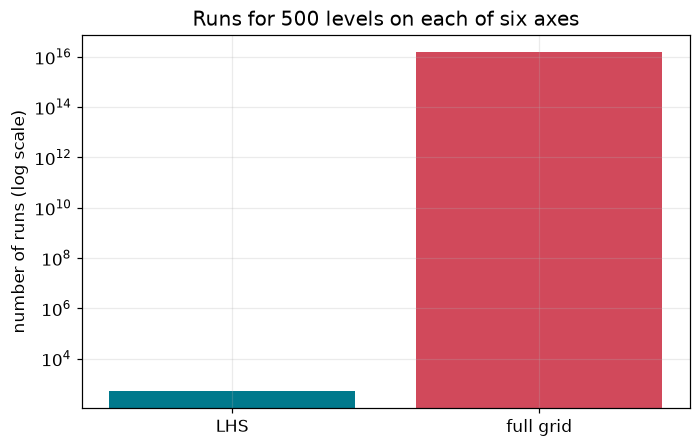
\includegraphics[width=0.57\linewidth]{lhs_budget.png}
\caption{Runs required to give all six inputs 500 distinct one-dimensional levels. The vertical scale is logarithmic.}
\label{fig:lhs}
\end{figure}

\section{Question 2: affine regression}
The baseline model is a global plane, $\hat y(\mathbf{x})=w_0+\sum_{j=1}^{6}w_jx_j$. With $Z=[\mathbf{1}\ X]$, the coefficients were calculated by solving the normal equations,
\begin{equation}
(Z^{\mathsf T}Z)\mathbf{w}=Z^{\mathsf T}\mathbf{y},
\end{equation}
using inputs on their natural scales except for $\log_{10}(\mathrm{Re})$. Table~\ref{tab:affine} lists the coefficients. The scikit-learn \texttt{LinearRegression} fit agreed to within $8.53\times10^{-14}$ in every coefficient and $7.99\times10^{-15}$ in test predictions. Both gave test RMSE $0.030767$ and $R^2=0.995256$.

\begin{table}[h]
\centering
\caption{Affine coefficients from the direct normal-equations solve; the library fit agrees at the displayed precision.}
\label{tab:affine}
\begin{tabular}{lr}
\toprule
Term & Coefficient \\
\midrule
Intercept & $-0.293009$ \\
Maximum camber $m$ & $13.848945$ \\
Camber position $p_{\mathrm{camber}}$ & $0.346723$ \\
Thickness $t$ & $0.599522$ \\
Angle of attack $\alpha_{\deg}$ & $0.125721$ \\
Mach number $M$ & $0.176949$ \\
$\log_{10}(\mathrm{Re})$ & $0.004182$ \\
\bottomrule
\end{tabular}
\end{table}

The affine model has a fixed complexity knob: its seven coefficients can express main effects, but no curvature or interactions. Its already high $R^2$ suggests that a linear global trend explains much of the response over the sampled domain. Its residual RMSE shows the cost of forcing every effect to remain linear. Coefficient magnitudes should not be compared as feature importance because these inputs have different units and ranges. Figure~\ref{fig:affine} displays the held-out predictions.

\begin{figure}[h]
\centering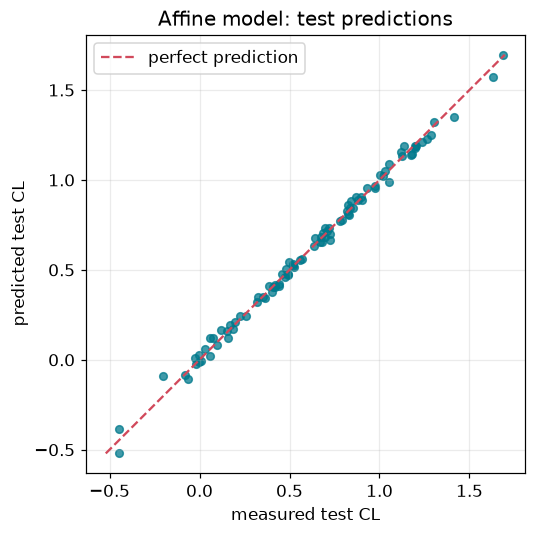
\includegraphics[width=0.53\linewidth]{affine_parity.png}
\caption{Measured and affine-predicted lift coefficient on the 93 test points.}
\label{fig:affine}
\end{figure}

\section{Question 3: quadratic features and ridge penalty}
The pure quadratic adds one square for each input, without cross terms:
\begin{equation}
\hat y(\mathbf{x})=w_0+\sum_{j=1}^{6}w_jx_j+\sum_{j=1}^{6}w_{j+6}x_j^2.
\end{equation}
Its design matrix has 13 columns. On natural input scales, $\kappa(Z^{\mathsf T}Z)=2.604\times10^{10}$; training-based min--max scaling reduces this to $1.496\times10^3$. This large improvement shows that coefficient estimation in normal equations is strongly affected by feature scale. Scaling does not resolve dependencies that are intrinsic to the features.

The ridge solution is
\begin{equation}
\mathbf{w}_{\lambda}=(Z^{\mathsf T}Z+\lambda I)^{-1}Z^{\mathsf T}\mathbf{y}.
\label{eq:ridge}
\end{equation}
Here the identity matrix includes the intercept coefficient, $w_0$. Table~\ref{tab:ridge} and Figure~\ref{fig:ridge} show the control-knob sweep.

\begin{table}[h]
\centering
\caption{Five-fold CV for scaled pure-quadratic ridge regression. Condition numbers use the full training design.}
\label{tab:ridge}
\begin{tabular}{rrr}
\toprule
$\lambda$ & Mean CV RMSE & $\kappa(Z^{\mathsf T}Z+\lambda I)$ \\
\midrule
$0$ & $0.034557$ & $1496.42$ \\
$10^{-4}$ & $0.034556$ & $1496.25$ \\
$10^{-2}$ & $\mathbf{0.034553}$ & $1479.46$ \\
$1$ & $0.054765$ & $697.54$ \\
$100$ & $0.306566$ & $13.93$ \\
\bottomrule
\end{tabular}
\end{table}

\begin{figure}[h]
\centering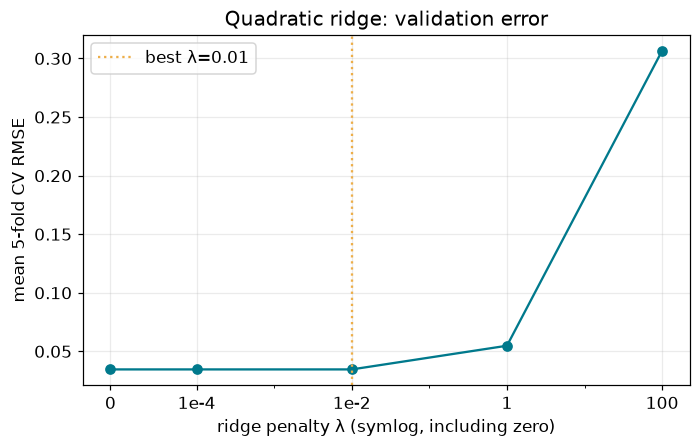
\includegraphics[width=0.62\linewidth]{ridge_cv.png}
\caption{Mean five-fold CV RMSE against the ridge penalty. A symmetric-log scale includes $\lambda=0$.}
\label{fig:ridge}
\end{figure}

CV selects $\lambda=0.01$, but its advantage over zero penalty is very small: mean CV RMSE changes by only $0.000004$. The corresponding test RMSE changes from $0.030816$ ($R^2=0.995241$) at $\lambda=0$ to $0.030776$ ($R^2=0.995254$) at $\lambda=0.01$. Thus this dataset offers little evidence that substantial regularization is needed for the quadratic fit. In contrast, $\lambda=100$ makes the system much better conditioned while increasing CV RMSE to $0.306566$, making the model considerably less desirable as numerical stability alone is not the objective. Adding $\lambda I$ shrinks poorly determined eigendirections of the Hessian of the least-squares objective $Z^{\mathsf T}Z$ most strongly (directions that minimization of the least-squares objective is not sensitive too are driven to zero). This reduces overfitting and sensitivity to training-set fluctuations as features in the training set that may not be very meaningful are not modeled as strongly. The trade-off is that coefficients are biased toward zero; too much shrinkage underfits.

\section{Question 4: Gaussian RBF spread}
The Gaussian RBF interpolation model places one basis function at each training point:
\begin{equation}
\hat y(\tilde{\mathbf{x}})=\sum_{j=1}^{N}a_j
\exp\!\left[-\lambda\|\tilde{\mathbf{x}}-\tilde{\mathbf{x}}_j\|_2^2\right],\qquad
\Phi_{ij}=\exp\!\left[-\lambda\|\tilde{\mathbf{x}}_i-\tilde{\mathbf{x}}_j\|_2^2\right].
\end{equation}
The weights solve $\Phi\mathbf a=\mathbf y$. The same functions are then evaluated at a query point. Scaling is essential because Euclidean distance should not be dominated by the input with the largest numerical units. In SciPy's \texttt{RBFInterpolator}, the Gaussian parameter is $\epsilon=\sqrt{\lambda}$; the default polynomial tail in was disabled so this matches the lecture model.

The $e^{-1}$ influence radius is $1/\sqrt{\lambda}$. Table~\ref{tab:rbf} and Figure~\ref{fig:rbf} show that this spread knob has a much sharper effect than the small ridge penalties. All stably solved Gaussian interpolants can closely reproduce their training outputs; validation error is needed to compare predictions between centers.

\begin{table}[h]
\centering
\caption{Five-fold CV across broad and narrow Gaussian RBF spreads.}
\label{tab:rbf}
\begin{tabular}{rr@{\hspace{2em}}rr}
\toprule
$\lambda$ & Mean CV RMSE & $\lambda$ & Mean CV RMSE \\
\midrule
$10^{-6}$ & $1.962631$ & $10^{-1}$ & $0.000446$ \\
$10^{-5}$ & $1.609502$ & $1$ & $0.013047$ \\
$10^{-4}$ & $0.573025$ & $10$ & $0.304625$ \\
$10^{-3}$ & $0.045375$ & $100$ & $0.796724$ \\
$\mathbf{10^{-2}}$ & $\mathbf{0.000321}$ & $1000$ & $0.800736$ \\
\bottomrule
\end{tabular}
\end{table}

\begin{figure}[h]
\centering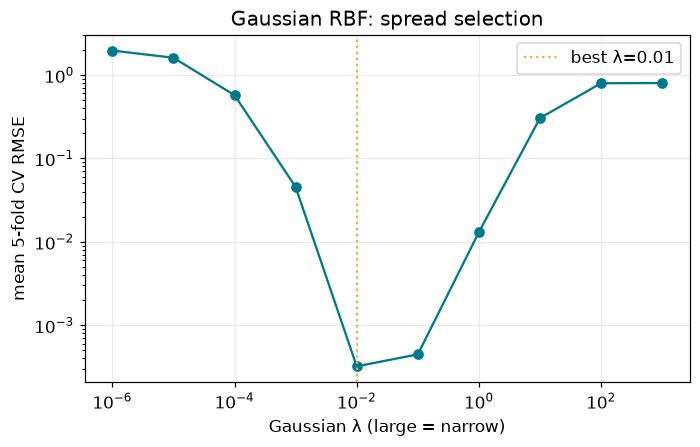
\includegraphics[width=0.62\linewidth]{rbf_cv.png}
\caption{Mean five-fold CV RMSE against Gaussian spread $\lambda$. Smaller $\lambda$ gives wider, more overlapping basis functions.}
\label{fig:rbf}
\end{figure}

CV selects $\lambda=0.01$ and the refitted test RMSE is $0.000273$ ($R^2$ rounds to $1.000000$). For $\lambda\leq10^{-3}$, broad Gaussian columns become nearly alike as $\Phi$ approaches an all-ones matrix; the ill-conditioned interpolation solve and poor validation scores reveal the wide-spread limit. At large $\lambda$, functions are narrow and have little influence between centers, so test locations receive inadequate interpolation. The selected value gives enough overlap to represent the smooth response to the inputs while avoiding the very poor CV behavior at either extreme. The exact-interpolation construction remains sensitive to conditioning, especially when functions are broad; the low held-out error demonstrates good performance on this split rather than a guarantee of numerical robustness on other data.

\section{Question 5: neural-network width}
For one hidden layer with ReLU activation $g$, the network has the form
\begin{equation}
\hat y(\tilde{\mathbf{x}})=b_0+\sum_{h=1}^{H}v_hg(\mathbf a_h^{\mathsf T}\tilde{\mathbf{x}}+b_h).
\end{equation}
There are six input nodes, $H$ hidden nodes, and one output node. Unlike RBF centers fixed at training points, the network learns its hidden-unit weights and biases. Width $H$ is the principal capacity knob in this experiment; the fitting procedure uses the \texttt{lbfgs} solver, maximum 5000 iterations, random initialization, and scikit-learn's default $L_2$ penalty $\alpha=10^{-4}$ fixed. A width-$H$ network has $8H+1$ trainable weights and biases, so the selected $H=128$ model has 1025 parameters.

\begin{table}[h]
\centering
\caption{Mean five-fold validation and fitting-fold training RMSE by hidden width.}
\label{tab:ann}
\begin{tabular}{rrr}
\toprule
$H$ & Mean validation RMSE & Mean training RMSE \\
\midrule
$2$ & $0.034901$ & $0.033919$ \\
$8$ & $0.028015$ & $0.027193$ \\
$32$ & $0.018514$ & $0.015688$ \\
$64$ & $0.013183$ & $0.010264$ \\
$\mathbf{128}$ & $\mathbf{0.010139}$ & $0.008167$ \\
$256$ & $0.012121$ & $0.009952$ \\
\bottomrule
\end{tabular}
\end{table}

\begin{figure}[h]
\centering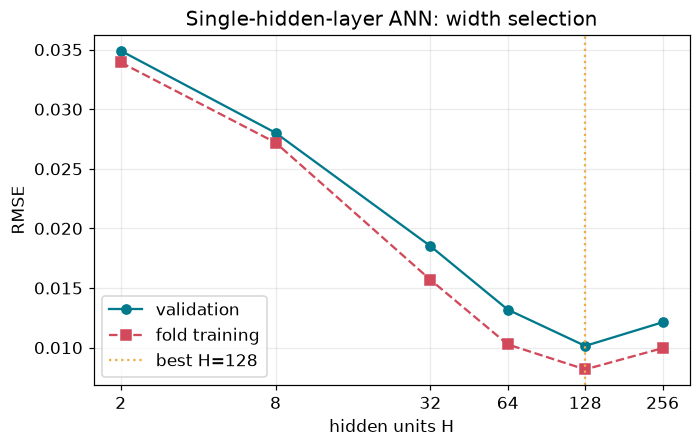
\includegraphics[width=0.62\linewidth]{ann_width_cv.png}
\caption{Network validation and training RMSE as the single hidden layer widens.}
\label{fig:ann}
\end{figure}

The small network has high training and validation error, consistent with insufficient capacity. Validation error then falls through $H=128$ and rises at $H=256$; the train--validation gap grows slightly. This is the first observed degradation in generalization as width increases. Since training error also rises at 256, the result is not clean proof of classical overfitting alone: nonconvex optimization and the fixed random initialization may also contribute. CV therefore selects $H=128$ rather than assuming that wider is always better. The selected network has test RMSE $0.010782$ and $R^2=0.999417$.

\section{Question 6: Kriging correlation and uncertainty}
\subsection{Manual ordinary Kriging on 25 training points}
The lecture model writes $Y(\tilde{\mathbf{x}})=\beta+Z(\tilde{\mathbf{x}})$, with constant mean $\beta$ and zero-mean correlated departure $Z$. For isotropic Gaussian correlation,
\begin{equation}
R_{ij}=\exp\!\left[-\theta\|\tilde{\mathbf{x}}_i-\tilde{\mathbf{x}}_j\|_2^2\right].
\end{equation}
Generalized least squares estimates the mean, and correlation with a new point predicts its departure from that mean:
\begin{equation}
\hat\beta=\frac{\mathbf1^{\mathsf T}R^{-1}\mathbf y}{\mathbf1^{\mathsf T}R^{-1}\mathbf1},\qquad
\hat y(\tilde{\mathbf{x}}_*)=\hat\beta+\mathbf r^{\mathsf T}R^{-1}(\mathbf y-\hat\beta\mathbf1).
\label{eq:kriging}
\end{equation}
Here $r_i=\exp[-\theta\|\tilde{\mathbf{x}}_i-\tilde{\mathbf{x}}_*\|_2^2]$. The implementation uses linear solves to apply $R^{-1}$ without explicitly forming the inverse. The baseline $\hat\beta$ is the unconditional constant mean; the correlation-weighted residual term supplies the local adjustment. The predictor is linear and unbiased under this model because its effective weights sum to one. That claim is conditional on the assumed correlation and mean of the response.

\begin{table}[h]
\centering
\caption{Conditioning of the 25-point correlation matrix, with and without a $10^{-6}$ diagonal nugget.}
\label{tab:kriging-cond}
\begin{tabular}{rrr}
\toprule
$\theta$ & $\kappa(R)$ & $\kappa(R+10^{-6}I)$ \\
\midrule
$10^{-3}$ & $1.168\times10^{10}$ & $2.492\times10^{7}$ \\
$10^{-2}$ & $1.050\times10^{8}$ & $2.003\times10^{7}$ \\
$10^{-1}$ & $5.374\times10^{5}$ & $5.250\times10^{5}$ \\
$1$ & $1.446\times10^{3}$ & $1.446\times10^{3}$ \\
$10$ & $11.679$ & $11.679$ \\
$100$ & $1.430$ & $1.430$ \\
\bottomrule
\end{tabular}
\end{table}

\begin{figure}[h]
\centering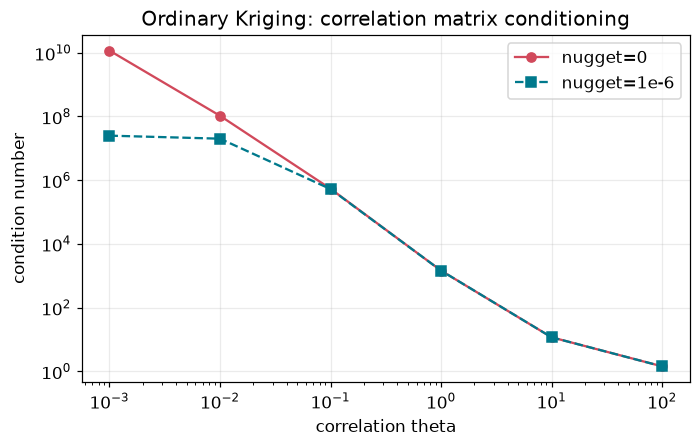
\includegraphics[width=0.62\linewidth]{kriging_condition.png}
\caption{The isotropic correlation rate $\theta$ changes numerical conditioning. A nugget mainly helps the strongly correlated, small-$\theta$ end.}
\label{fig:kriging-cond}
\end{figure}

This is a conditioning experiment, so no scalar $\theta$ is selected as a final predictor. At $\theta=10^{-3}$, nearly all points are highly correlated and $\kappa(R)=1.168\times10^{10}$; adding a $10^{-6}$ nugget reduces it to $2.492\times10^7$, though this modifies the covariance and may break exact interpolation. At $\theta=100$, distinct points are much less correlated and $R$ approaches the identity. A new point away from training locations then reverts quickly toward $\hat\beta$, with larger predictive uncertainty. The observed nearly zero 25-point training interpolation errors across the sweep is expected since ordinary Kriging exactly interpolates the training outputs. These near-zero training errors only confirm interpolation; they cannot determine which $\theta$ will predict new locations best; validation or likelihood is needed for that purpose.

\subsection{Full-data Gaussian process}
\begin{figure}[h]
\centering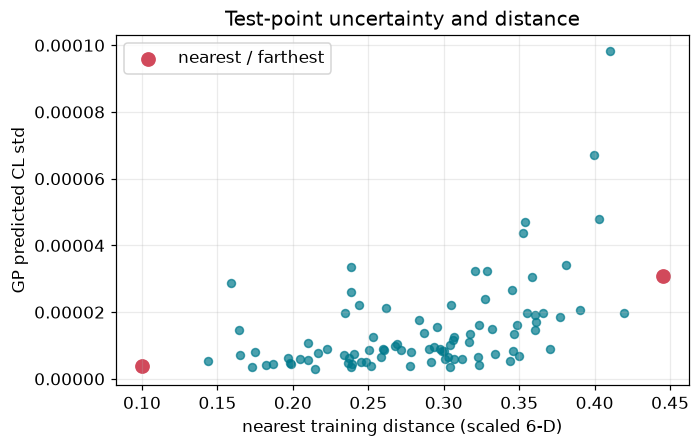
\includegraphics[width=0.62\linewidth]{gp_uncertainty.png}
\caption{Predicted GP standard deviation versus each test point's Euclidean distance to its nearest training point in scaled input space.}
\label{fig:gp-uncertainty}
\end{figure}

The final GP uses all 407 scaled training points and an anisotropic RBF kernel, with separate length scales $\ell_j$ fitted by marginal likelihood. Its \texttt{normalize\_y=True} setting centers and rescales the training responses during fitting; this library mean treatment differs from the manual GLS estimate in Eq.~\eqref{eq:kriging}. The covariance kernel is
\begin{equation}
k(\tilde{\mathbf{x}},\tilde{\mathbf{x}}')=\sigma_f^2
\exp\!\left[-\sum_{j=1}^{6}\frac{(\tilde x_j-\tilde x'_j)^2}{2\ell_j^2}\right].
\label{eq:gp-kernel}
\end{equation}
The fitted kernel was $12.7^2\!\times\mathrm{RBF}([5.02,1.76,12.1,5.13,1.69,1000])$ in input order. Its length scales correspond to direction-specific correlation rates $\theta_j=1/(2\ell_j^2)$; the sixth length scale reached its imposed upper bound of 1000. Across the entire scaled $\log_{10}(\mathrm{Re})$ range, this coordinate alone contributes a correlation factor of approximately $\exp[-1/(2\cdot1000^2)]=0.9999995$. Thus the fitted data support almost no variation in $C_L$ along Reynolds number after accounting for the other inputs. This is likely a dataset-specific finding, not a general aerodynamic law. The optimizer issued three convergence warnings across its restarts; the fit completed, but a bound-hitting length scale.

The GP achieved test RMSE $0.000038$ and $R^2$ rounding to $1.000000$. The nearest test point to any training point was at scaled six-dimensional distance $0.099934$, with predicted standard deviation $0.000004$; the farthest was at $0.445221$, with predicted standard deviation $0.000031$. Figure~\ref{fig:gp-uncertainty} shows all test points. The greater uncertainty at the farthest point is consistent with less nearby information, but GP uncertainty depends on the entire training geometry and the learned length scales, not just ordinary Euclidean distance. These standard deviations are conditional on the fitted GP model.

\clearpage
\section{Bonus: comparing surrogate families}
\begin{table}[h]
\centering
\caption{Held-out performance of the fitted families. $R^2$ values printed as $1.000000$ are rounded, not exact unity.}
\label{tab:comparison}
\begin{tabular}{p{0.23\linewidth}p{0.31\linewidth}rrc}
\toprule
Family & Main control knob & Test RMSE & Test $R^2$ & Native UQ? \\
\midrule
Affine regression & Fixed seven-parameter form & $0.030767$ & $0.995256$ & No \\
Quadratic + ridge & $\lambda=0.01$ & $0.030776$ & $0.995254$ & No \\
Gaussian RBF & Spread $\lambda=0.01$ & $0.000273$ & $1.000000$ & No \\
One-layer ANN & Width $H=128$ & $0.010782$ & $0.999417$ & No \\
Kriging / GP & Six learned length scales & $0.000038$ & $1.000000$ & Yes \\
\bottomrule
\end{tabular}
\end{table}

The test ranking reinforces that complexity is useful only when its control knob fits the response structure. The quadratic model adds curvature but almost no test benefit over the affine baseline; the absence of interaction terms limits its expressiveness. The RBF gains two orders of magnitude in accuracy by using many local basis functions with the right spread, though the Gaussian kernel solve can be numerically fragile when the spread is very broad. The ANN improves on the global polynomials, but widening it past 128 units worsens validation performance in this comparison structure. Kriging obtains the lowest test error and uniquely supplies a predictive standard deviation, at the price of a more expensive covariance fit and assumptions underlying its uncertainty estimates.

For predicting $C_L$ on this sample domain, the Affine model is likely sufficient with its test RMSE and saves on computational complexity. It is highly unlikely that this model would perform outside the bounds of the sample domain or if the sample domain was extended to more dynamic areas. Otherwise, the GP model would be recommended for this problem since it supplies uncertainty information and had the lowest test RMSE.

\end{document}
